% Source: Code/ML_overlay/ir_rgb_registration/paper/ml_overlay_report_materials/ir_rgb_registration_report/figures/fig_training_curves.tex
\documentclass[tikz,border=10pt]{standalone}
\usepackage{tikz}
\usetikzlibrary{calc}
\usepackage{pgfplots}
\pgfplotsset{compat=1.18}

\definecolor{Garnet}{RGB}{115, 0, 10}
\definecolor{Rose}{RGB}{204, 46, 64}
\definecolor{Atlantic}{RGB}{70, 106, 159}
\definecolor{Congaree}{RGB}{31, 65, 77}
\definecolor{Horseshoe}{RGB}{101, 120, 11}
\definecolor{Black30}{RGB}{199, 199, 199}
\definecolor{Black70}{RGB}{92, 92, 92}

\begin{document}
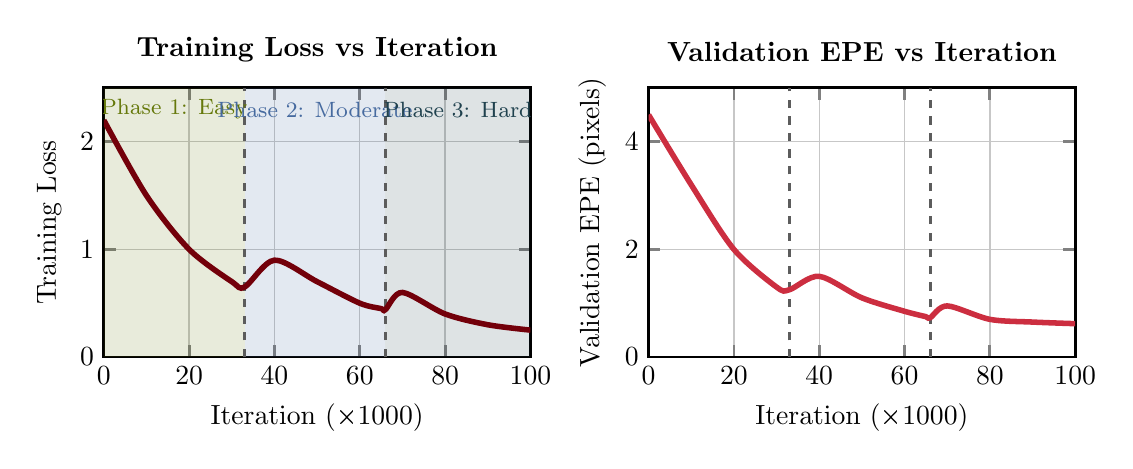
\begin{tikzpicture}

% Left plot: Training Loss
\begin{axis}[
    name=loss,
    width=7cm,
    height=5cm,
    xlabel={Iteration (×1000)},
    ylabel={Training Loss},
    xmin=0, xmax=100,
    ymin=0, ymax=2.5,
    grid=major,
    grid style={Black30, line width=0.5pt},
    legend pos=north east,
    title={Training Loss vs Iteration},
    title style={font=\bfseries},
    axis line style={line width=1pt},
    tick style={line width=1pt}
]

% Phase backgrounds
\fill[Horseshoe, opacity=0.15] (axis cs:0,0) rectangle (axis cs:33,2.5);
\fill[Atlantic, opacity=0.15] (axis cs:33,0) rectangle (axis cs:66,2.5);
\fill[Congaree, opacity=0.15] (axis cs:66,0) rectangle (axis cs:100,2.5);

% Phase dividers
\draw[dashed, Black70, line width=1pt] (axis cs:33,0) -- (axis cs:33,2.5);
\draw[dashed, Black70, line width=1pt] (axis cs:66,0) -- (axis cs:66,2.5);

% Training loss curve
\addplot[Garnet, line width=2pt, smooth] coordinates {
    (0,2.2) (10,1.5) (20,1.0) (30,0.7)
    (33,0.65) (40,0.9) (50,0.7) (60,0.5) (65,0.45)
    (66,0.44) (70,0.6) (80,0.4) (90,0.3) (100,0.25)
};

% Phase labels
\node[font=\footnotesize, Horseshoe] at (axis cs:16.5,2.3) {Phase 1: Easy};
\node[font=\footnotesize, Atlantic] at (axis cs:49.5,2.3) {Phase 2: Moderate};
\node[font=\footnotesize, Congaree] at (axis cs:83,2.3) {Phase 3: Hard};

\end{axis}

% Right plot: Validation EPE
\begin{axis}[
    name=epe,
    at={($(loss.east)+(1.5cm,0)$)},
    anchor=west,
    width=7cm,
    height=5cm,
    xlabel={Iteration (×1000)},
    ylabel={Validation EPE (pixels)},
    xmin=0, xmax=100,
    ymin=0, ymax=5,
    grid=major,
    grid style={Black30, line width=0.5pt},
    legend pos=north east,
    title={Validation EPE vs Iteration},
    title style={font=\bfseries},
    axis line style={line width=1pt},
    tick style={line width=1pt}
]

% Phase dividers
\draw[dashed, Black70, line width=1pt] (axis cs:33,0) -- (axis cs:33,5);
\draw[dashed, Black70, line width=1pt] (axis cs:66,0) -- (axis cs:66,5);

% Validation EPE curve
\addplot[Rose, line width=2pt, smooth] coordinates {
    (0,4.5) (10,3.2) (20,2.0) (30,1.3)
    (33,1.25) (40,1.5) (50,1.1) (60,0.85) (65,0.75)
    (66,0.73) (70,0.95) (80,0.7) (90,0.65) (100,0.62)
};

\end{axis}

\end{tikzpicture}
\end{document}
